%===============================================================================
% CHAPTER 3: SYSTEM ARCHITECTURE & DESIGN
%===============================================================================
\chapter{System Architecture and Design}
\label{ch:architecture}

\section{Architectural Overview}
\label{sec:arch-overview}

This system implements a \textit{Web2.5 hybrid architecture} that decouples identity
management (Web2/cloud) from vote consensus (Web3/DLT). The architecture comprises
five logical layers:

\begin{figure}[H]
\centering
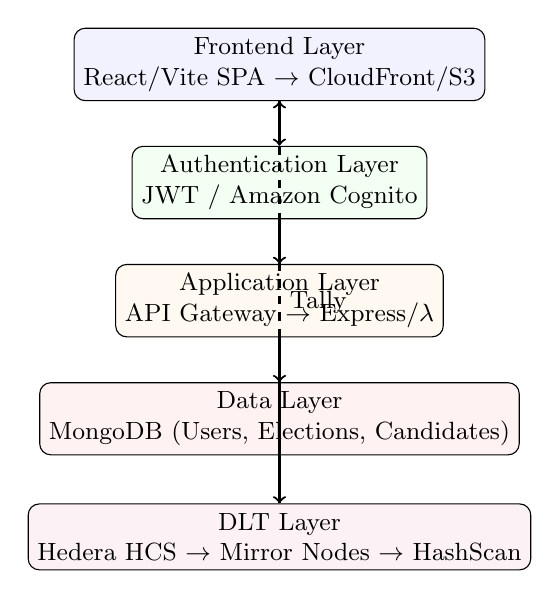
\begin{tikzpicture}[node distance=1.5cm, every node/.style={font=\small, align=center}]
\node[draw, rounded corners, fill=blue!5] (frontend) {Frontend Layer\\React/Vite SPA $\rightarrow$ CloudFront/S3};
\node[draw, rounded corners, fill=green!5, below of=frontend] (auth) {Authentication Layer\\JWT / Amazon Cognito};
\node[draw, rounded corners, fill=orange!5, below of=auth] (app) {Application Layer\\API Gateway $\rightarrow$ Express/$\lambda$};
\node[draw, rounded corners, fill=red!5, below of=app] (data) {Data Layer\\MongoDB (Users, Elections, Candidates)};
\node[draw, rounded corners, fill=purple!5, below of=data] (dlt) {DLT Layer\\Hedera HCS $\rightarrow$ Mirror Nodes $\rightarrow$ HashScan};

\draw[->, thick] (frontend) -- (auth);
\draw[->, thick] (auth) -- (app);
\draw[->, thick] (app) -- (data);
\draw[->, thick] (app) -- (dlt);
\draw[->, thick, dashed] (dlt) -- node[right]{Tally} (frontend);
\end{tikzpicture}
\caption{High-level system architecture}
\label{fig:architecture}
\end{figure}

\section{Component Architecture}
\label{sec:components}

\subsection{Frontend Components}
\label{sec:frontend-components}

\begin{table}[H]
\centering
\caption{Frontend Component Responsibilities}
\label{tab:frontend-components}
\begin{tabular}{@{}ll@{}}
\toprule
\textbf{Component} & \textbf{Responsibility} \\
\midrule
LandingPage & Public information, election overview \\
Login / Register & Authentication forms, JWT acquisition \\
ManifestoDashboard & Candidate profiles, manifestos, issues, evidence \\
VoterBooth & Ballot casting, transaction confirmation \\
AdminConsole & Election management, candidate/voter CRUD, stats \\
App.jsx route guards & Role-based navigation checks \\
\midrule
\end{tabular}
\end{table}

\subsection{Backend Services}
\label{sec:backend-services}

\begin{table}[H]
\centering
\caption{Backend Service Responsibilities}
\label{tab:backend-services}
\begin{tabular}{@{}ll@{}}
\toprule
\textbf{Module} & \textbf{Responsibility} \\
\midrule
server.js & Express app, middleware, routing, Hedera init \\
controllers/auth & Login, JWT issuance \\
controllers/election & Election lifecycle, candidate listing \\
controllers/vote & Vote casting, verification, results \\
controllers/admin & Admin-only CRUD for all entities \\
server.js Hedera client & Hedera SDK client and HCS submission \\
lib/voteErrors & Hedera error-message mapping \\
controllers/auth.js & Login and JWT issuance \\
models/* & MongoDB schemas (User, Election, Candidate, Vote, etc.) \\
\midrule
\end{tabular}
\end{table}

\subsection{Data Models}
\label{sec:data-models}

\begin{figure}[H]
\centering
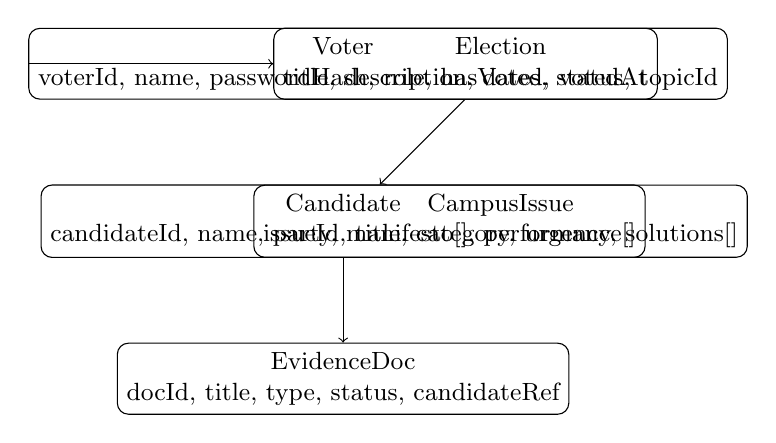
\begin{tikzpicture}[node distance=2cm, every node/.style={font=\small, align=center}]
\node[draw, rectangle, rounded corners] (voter) {Voter\\voterId, name, passwordHash, role, hasVoted, votedAt};
\node[draw, rectangle, rounded corners, right of=voter] (election) {Election\\title, description, dates, status, topicId};
\node[draw, rectangle, rounded corners, below of=voter] (candidate) {Candidate\\candidateId, name, party, manifesto[], performance[]};
\node[draw, rectangle, rounded corners, right of=candidate] (issue) {CampusIssue\\issueId, title, category, urgency, solutions[]};
\node[draw, rectangle, rounded corners, below of=candidate] (evidence) {EvidenceDoc\\docId, title, type, status, candidateRef};

\draw[->] (voter) -- (election);
\draw[->] (election) -- (candidate);
\draw[->] (candidate) -- (evidence);
\end{tikzpicture}
\caption{MongoDB data model relationships}
\label{fig:data-model}
\end{figure}

\section{Vote Transaction Lifecycle}
\label{sec:vote-flow}

The critical vote submission flow ensures atomic coordination between the database
(duplicate prevention) and the ledger (immutability):

\begin{enumerate}
    \item \textbf{Authentication:} Voter logs in $\rightarrow$ JWT issued with \texttt{sub=voterId}, \texttt{role=Voters}
    \item \textbf{Manifesto Review:} Frontend fetches \texttt{/api/manifesto/overview} $\rightarrow$ displays candidates, issues, evidence
    \item \textbf{Vote Submission:} POST \texttt{/castVote} with \texttt{\{candidateId\}} + JWT
    \item \textbf{Validation:} Middleware verifies JWT, checks \texttt{role=Voters}
    \item \textbf{Atomic Claim:} \texttt{findOneAndUpdate(\{voterId, hasVoted:false\}, \{hasVoted:true, votedAt:now\})}
    \item \textbf{HCS Submit:} \texttt{TopicMessageSubmitTransaction\{topicId, message:JSON(candidateId, timestamp)\}}
    \item \textbf{Rollback on Failure:} If HCS fails $\rightarrow$ revert voter \texttt{hasVoted=false}
    \item \textbf{Response:} Return \texttt{transactionId}, \texttt{status} to frontend
    \item \textbf{Tallying:} Frontend queries mirror node \texttt{/api/v1/topics/\{topicId\}/messages} $\rightarrow$ aggregate
    \item \textbf{Audit:} Voter clicks HashScan link with \texttt{transactionId} for public verification
\end{enumerate}

\begin{lstlisting}[style=codeStyle, caption=Atomic vote claim with HCS rollback, label=lst:vote-atomic]
const voter = await Voter.findOneAndUpdate(
  { voterId: voterId, hasVoted: false },
  { hasVoted: true, votedAt: new Date() },
  { returnDocument: 'after' }
);

if (!voter) {
  return res.status(403).json({ error: "Already voted or not found" });
}

try {
  const txResponse = await new TopicMessageSubmitTransaction({
    topicId,
    message: JSON.stringify({ candidateId, timestamp: new Date().toISOString() })
  }).execute(client);
  const receipt = await txResponse.getReceipt(client);

  res.json({ transactionId: txResponse.transactionId.toString(), status: receipt.status.toString() });
} catch (hederaErr) {
  await Voter.findOneAndUpdate(
    { voterId: voterId },
    { hasVoted: false, votedAt: null }
  );
  return res.status(502).json({ error: "Ledger submission failed, vote not recorded" });
}
\end{lstlisting}

\section{Security Architecture}
\label{sec:security-arch}

\begin{table}[H]
\centering
\caption{Security Controls by Layer}
\label{tab:security-controls}
\begin{tabular}{@{}lll@{}}
\toprule
\textbf{Layer} & \textbf{Control} & \textbf{Implementation} \\
\midrule
Transport & TLS in production & Deployment requirement; local development uses HTTP \\
AuthN & JWT (shared secret) & \texttt{jsonwebtoken}, bcrypt password hash \\
AuthZ & Role-based & Middleware \texttt{requireRole("Voters"/"Admins")} \\
Vote Integrity & Atomic DB+HCS & Optimistic lock + rollback on HCS failure \\
Replay Protection & JWT expiry & JWT \texttt{exp}; HCS timestamp is an audit field \\
Audit Trail & Immutable & HCS topic + Mirror node history \\
Input Validation & Route-level checks & Required fields and Mongoose lookups in current prototype \\
Rate Limiting & Not implemented & Production deployment requirement \\
\midrule
\end{tabular}
\end{table}

\section{Deployment Architecture}
\label{sec:deployment-arch}

\begin{figure}[H]
\centering
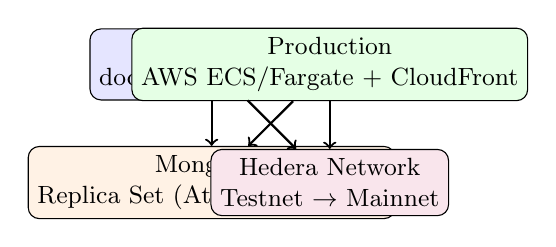
\begin{tikzpicture}[node distance=1.5cm, every node/.style={font=\small, align=center}]
\node[draw, rounded corners, fill=blue!10] (dev) {Development\\docker-compose.yml};
\node[draw, rounded corners, fill=green!10, right of=dev] (prod) {Production\\AWS ECS/Fargate + CloudFront};
\node[draw, rounded corners, fill=orange!10, below of=dev] (db) {MongoDB\\Replica Set (Atlas/Self-hosted)};
\node[draw, rounded corners, fill=purple!10, below of=prod] (hedera) {Hedera Network\\Testnet $\rightarrow$ Mainnet};

\draw[->, thick] (dev) -- (db);
\draw[->, thick] (dev) -- (hedera);
\draw[->, thick] (prod) -- (db);
\draw[->, thick] (prod) -- (hedera);
\end{tikzpicture}
\caption{Deployment topology}
\label{fig:deployment}
\end{figure}

Docker Compose orchestrates three services: \texttt{backend} (Node.js), \texttt{frontend} (Nginx + React build), and \texttt{mongodb}. Production replaces Compose with ECS services behind an Application Load Balancer, with CloudFront for global CDN.
